% SPDX-License-Identifier: MIT
% Preprint: ntpstats, an open toolkit for validating, evaluating and studying network time synchronisation.
% Build: make   (needs pdflatex and bibtex; numbers and figures come from experiments.py and make_tables.py)
\documentclass[11pt,a4paper]{article}

\usepackage[T1]{fontenc}
\usepackage[utf8]{inputenc}
\usepackage{newtxtext,newtxmath}
\usepackage[margin=25mm]{geometry}
\usepackage[expansion=false]{microtype}
\usepackage{graphicx}
\usepackage{booktabs}
\usepackage{tabularx}
\usepackage{amsmath}
\usepackage{enumitem}
\usepackage{xcolor}
\usepackage{tikz}
\usetikzlibrary{positioning,arrows.meta,fit}
\usepackage[font=small,labelfont=bf]{caption}
\usepackage[numbers,sort&compress]{natbib}
\usepackage{xurl}
\usepackage[hidelinks,pdfusetitle]{hyperref}
\usepackage[capitalise,noabbrev]{cleveref}

\setlist{itemsep=2pt,topsep=4pt}
\makeatletter\newcommand{\rows}[1]{\@@input #1 }\makeatother
\newcommand{\ntp}{\texttt{ntpstats}}
\newcommand{\micro}{\ensuremath{\upmu}}
\newcommand{\us}{\,\micro s}
\newcommand{\ns}{\,ns}
\newcommand{\ms}{\,ms}

\hypersetup{pdfauthor={Thiago de Freitas},pdfkeywords={network time synchronisation, NTP, PTP, frequency stability, Allan deviation, time error, clock synchronisation algorithms, reproducibility}}

\title{\ntp: an open toolkit for validating, evaluating\\ and studying network time synchronisation}
\author{Thiago de Freitas\\[2pt]
\small Independent researcher\\
\small ORCID \href{https://orcid.org/0009-0006-7749-1401}{0009-0006-7749-1401}\quad
GitHub \href{https://github.com/thiagodefreitas}{@thiagodefreitas}}
\date{Preprint, 3 October 2026\\[2pt]\small Software version 3.5.0, \href{https://doi.org/10.5281/zenodo.23070521}{doi:10.5281/zenodo.23070521}}

\begin{document}
\maketitle

\begin{abstract}
\noindent
The quality of network time synchronisation is a measurement problem: how far a clock is from its
reference, how stable it is, how much of the error the network contributes, and whether another
algorithm would do better. In practice, each of these questions is answered with separate tools and ad
hoc scripts, which makes results from different deployments and different papers hard to compare. We
describe \ntp, an open-source Python toolkit that joins the steps of such an evaluation. It reads the
logs of current time daemons (ntpd, NTPsec, chrony, linuxptp, ntpd-rs), packet captures of NTP, PTP,
NTP over PTP and client-server PTP, GNSS receiver and time-transfer data, laboratory counters and
network-simulator output, and maps them onto one data model with a single sign convention. On this
model it computes the frequency-stability statistics of NIST SP~1065 with confidence intervals from
the exact equivalent degrees of freedom of the discrete power-law noise model, the time-error metrics
of ITU-T G.8260, power-law noise fits, N-cornered-hat separation and holdover predictions. A research
bench scores clock-synchronisation estimators against simulated clocks with known truth, including
replayed network delays, PTP exchanges and chains of boundary clocks. We report the validation of the
statistics against the published NIST test suites (largest relative deviation $2.8\times10^{-7}$ at seven
printed digits), a Monte Carlo study of interval coverage, a benchmark of thirteen reference
estimators, and a study of time-error accumulation in boundary-clock chains, all reproducible from a
seeded script.
\end{abstract}

\noindent\textbf{Keywords:} network time synchronisation; NTP; PTP; frequency stability; Allan deviation;
time error; clock-synchronisation algorithms; reproducible research.

\section{Introduction}\label{sec:intro}

Packet networks distribute time to almost every computer, to mobile networks, to trading systems
and to power grids. Most hosts use the Network Time Protocol (NTP) \citep{mills1991,rfc5905}, increasingly
authenticated with Network Time Security (NTS) \citep{rfc8915}; telecom and industrial networks use the
Precision Time Protocol (PTP) of IEEE~1588 \citep{ieee1588}. The protocols have matured, and the
accuracy that is achievable now ranges from milliseconds over the Internet to nanoseconds with hardware
time stamps and on-path support. Assessing that accuracy has not become easier. An operator who wants
evidence that a fleet stays within a regulatory limit, an engineer qualifying a boundary clock, and a
researcher proposing a new synchronisation algorithm all need the same chain of steps: extract the
offsets and delays from what the system recorded, place them on a common time base and sign
convention, compute statistics with defensible uncertainties, and compare the result with a limit or
with an alternative.

These steps are well understood individually. The statistics of frequency stability go back to Allan
\citep{allan1966} and Barnes et al.\ \citep{barnes1971}, and are collected in NIST SP~1065 \citep{riley2008}
and IEEE Std~1139 \citep{ieee1139}. Packet-network time error is defined in ITU-T G.810 and G.8260
\citep{g810,g8260}, with limits in G.8271.1 and G.8273.2 \citep{g8271_1,g8273_2}. Synchronisation
algorithms are documented in the NTP specification \citep{rfc5905} and in the research literature
\citep{veitch2009,geng2018,li2020sundial}. What is missing is a common, open implementation that
connects the data that systems actually produce with these definitions. Stability programs such as
Stable32 \citep{stable32}, TimeLab \citep{timelab} and the \texttt{allantools} library \citep{allantools}
expect a clean, uniformly sampled phase or frequency record; daemons and their plotting tools
\citep{ntpviz} report their own state rather than evaluate it; PTP time error is usually measured with
vendor instruments and closed analysis software. Papers on synchronisation algorithms tend to come with
one-off evaluation code, so their numbers rarely share definitions or test conditions.

\ntp{} addresses this gap. It began in 2012 as a Google Summer of Code project for the NTP Project of
the Network Time Foundation and was rewritten from 2026 as a validation, evaluation and study toolkit.
This paper describes the design of version 3.5.0 and reports its validation and a set of experiments
that the toolkit makes reproducible. The contributions are:
\begin{enumerate}[label=(\roman*)]
\item a data model and input layer that read 26 built-in formats, from daemon logs and packet captures
  (NTP, PTP, NTP over PTP \citep{rfc10030}, client-server PTP) to GNSS receivers, laboratory counters,
  BIPM and IGS products, Internet measurement platforms and network simulators, with one documented
  sign convention (\cref{sec:data});
\item implementations of the NIST SP~1065 stability statistics with confidence intervals from the
  exact equivalent degrees of freedom (EDF) of the discrete power-law noise model, together with ITU-T
  time-error metrics, power-law noise fitting, N-cornered-hat separation and holdover prediction
  (\cref{sec:stats});
\item a research bench that scores synchronisation estimators against simulated clocks with known
  truth, including replayed network delays, exchange-level PTP and boundary-clock chains, and thirteen
  reference estimators (\cref{sec:bench});
\item a validation against published reference values and a Monte Carlo study of interval coverage
  (\cref{sec:validation});
\item experiments on estimator accuracy, PTP clients, boundary-clock chains and public servers, all
  generated by one seeded script published with the paper (\cref{sec:experiments}).
\end{enumerate}

\section{Background}\label{sec:background}

\subsection{Two-way time transfer and its limit}

An NTP client sends a request at its time $T_1$; the server receives it at $T_2$ and answers at $T_3$;
the client receives the answer at $T_4$. The offset and the round-trip delay are
\begin{equation}\label{eq:ntp}
\theta = \frac{(T_2 - T_1) + (T_3 - T_4)}{2}, \qquad \delta = (T_4 - T_1) - (T_3 - T_2),
\end{equation}
with $\theta$ the reference minus the local clock \citep{rfc5905}. If the one-way delays are $d_f$ and
$d_b$, the measured offset differs from the true one by $(d_f - d_b)/2$. Because $d_f, d_b \ge 0$ and
$d_f + d_b = \delta$, the error of a single exchange is bounded by $\delta/2$, and the true offset lies
in $[\theta - \delta/2, \theta + \delta/2]$. The bound is reached when all of the delay is on one side.
A constant asymmetry cannot be observed with two-way time stamps at all: it biases every estimate by
half its value. Queueing, on the other hand, varies from packet to packet, and the exchanges with the
smallest delay are the least affected. This is the idea behind the NTP clock filter \citep{rfc5905},
the regression of chrony \citep{chrony}, feed-forward clocks \citep{veitch2009} and the convex-hull
approach of Huygens \citep{geng2018}. PTP uses the same equations, with one-way Sync messages and
separate Delay\_Req exchanges in the end-to-end delay mechanism, and adds a correction field in which
transparent clocks report the queueing they measured \citep{ieee1588}. RFC~10030 carries NTP messages in
PTP event messages so that NTP can benefit from PTP hardware time stamping and from these corrections
\citep{rfc10030}.

\subsection{Frequency stability and its uncertainty}

Clock noise is commonly described by the power-law model of the one-sided spectral density of
fractional frequency, $S_y(f) = \sum_{\alpha=-2}^{2} h_\alpha f^\alpha$, whose five terms are white and
flicker phase modulation (PM, $\alpha = 2, 1$), white and flicker frequency modulation (FM, $\alpha = 0,
-1$) and random-walk FM ($\alpha=-2$) \citep{barnes1971}. The Allan deviation and its overlapping,
modified, Hadamard, total and Theo variants \citep{allan1966,allan1981,howe2000,howe2003theo,howe2006theoh}
estimate the stability at averaging time $\tau$ from phase data $x$ sampled at interval $\tau_0$; NIST
SP~1065 gives their definitions and test data \citep{riley2008}. Each estimate is a random variable. Its
confidence interval follows from a $\chi^2$ distribution whose equivalent degrees of freedom depend on
the estimator, the averaging factor $m = \tau/\tau_0$, the record length and the noise type
\citep{greenhall2003}. The noise type can be identified from the data with the lag-1 autocorrelation
\citep{riley2004}. A widely used shortcut, an error bar of $\sigma_y/\sqrt{n}$ for $n$ terms, ignores the
correlation between overlapping terms; \cref{sec:coverage} quantifies how much that matters.

\subsection{Time error in packet networks}

In telecom practice, the time error is $\mathrm{TE}(t) = $ local $-$ reference. ITU-T G.8260 defines
the maximum absolute time error max|TE|, the constant time error cTE, and the dynamic time error dTE,
split by a low-pass filter (0.1~Hz) into a low-frequency part dTE$_\mathrm{L}$, characterised by the
maximum time interval error (MTIE) and the time deviation (TDEV), and a high-frequency part dTE$_\mathrm{H}$
\citep{g8260}. G.8273.2 sets per-clock limits for boundary clocks in classes A to D, and G.8271.1 sets
network limits such as 1.1\us{} max|TE| at the end of a chain for applications that need 1.5\us{}
end-to-end \citep{g8273_2,g8271_1}.

\subsection{Related tools}\label{sec:related}

Stable32 \citep{stable32} and TimeLab \citep{timelab} are the reference desktop programs of the time and
frequency community; \texttt{allantools} \citep{allantools} provides the classical deviations in Python.
They analyse clean phase or frequency records and do not read daemon logs or packet captures, nor
address network effects or the time-error metrics of packet networks. NTPsec's \texttt{ntpviz}
\citep{ntpviz} plots percentiles of ntpd statistics files. OMNeT++ with INET \citep{omnetpp,inet} and
ns-3 \citep{ns3} simulate networks, including PTP models, but leave the statistical evaluation to the
user. Algorithm papers such as Huygens \citep{geng2018}, Sundial \citep{li2020sundial} and RADclock
\citep{veitch2009} report their own evaluations under their own conditions. \ntp{} is designed to
interoperate with these tools rather than replace them: it reads and writes Stable32 data files, offers
an \texttt{allantools}-compatible interface, and reads and writes OMNeT++ vector files and ns-3 text and
captures.

\section{Data model and inputs}\label{sec:data}

\subsection{One series type and one sign convention}

Every input becomes a \texttt{TimeSeries}: POSIX time stamps $t_i$, offsets $\theta_i$ in seconds,
optional per-sample columns (round-trip delay, dispersion, frequency, servo state, PTP correction,
GNSS quantisation error, and others) and a metadata dictionary that records the source, the peer and
any assumption made while parsing. Offsets always mean \emph{reference minus local}, the convention of
ntpd \citep{rfc5905}. Implementations disagree on this point: chrony's tracking and statistics logs and
linuxptp report local minus reference, RIPE Atlas reports local minus server, and the time-error
metrics of ITU-T use local minus reference. The parsers convert on import, following each
implementation's documentation, and the conversion is tested on the line layouts given in that
documentation. A consistency test simulates one NTP peer and writes it as ntpd \texttt{peerstats},
ntpd \texttt{rawstats}, chrony \texttt{measurements.log} and a packet capture; all four must read back
identically.

Irregular logs are placed on a uniform grid at their median sampling interval $\tau_0$. Grid points
inside gaps longer than a configurable multiple of $\tau_0$ are left empty and every estimator term
that touches them is dropped, so gaps are never bridged by interpolation, which would add exactly the
kind of smooth noise that the statistics are meant to measure. Time stamps from captures and bound
windows are parsed as exact integers or decimals, because a double-precision number cannot hold
nanoseconds at current POSIX epochs.

\subsection{Inputs}

\Cref{tab:inputs} groups the 26 built-in formats. Formats are detected from content, so most
commands need no format flag. Daemon logs cover the three NTP implementations in common use and the
linuxptp stack \citep{chrony,linuxptp,cochran2011}. Live sampling is available for chrony, ntpd,
ntpd-rs \citep{ntpdrs}, ptp4l, Meta's \texttt{ptpcheck} \citep{fbtime} and gpsd \citep{gpsd}.

The capture reader decodes NTP versions~3 to~5 and IEEE~1588 version 2 and 2.1 over UDP and Ethernet. For
PTP it reconstructs the offset and mean path delay of each master and slave pair from Sync, Follow\_Up,
Delay\_Req and Delay\_Resp (or the peer-delay messages), applying the correction fields, and it takes the
UTC offset from Announce messages. For NTP over PTP \citep{rfc10030} it applies the corrections of the
request and the response as the RFC specifies,
\begin{equation}
\theta_c = \theta + \frac{c_\mathrm{rs} - c_\mathrm{rq}}{2}, \qquad
\delta_c = \delta - (c_\mathrm{rs} + c_\mathrm{rq} - d_\mathrm{rs} - d_\mathrm{rq})(1 - 10^{-4}),
\end{equation}
where $c$ are the network corrections and $d$ the frame durations, and it rejects corrections that the
RFC says must not be applied. Client-server PTP exchanges (CSPTP), as implemented experimentally in
ntpd-rs, are reconstructed with all four time stamps and their correction fields. Interleaved NTP
responses \citep{rfc9769} are recognised, and the offset is recomputed with the precise transmit time
stamp carried in the following response.

GNSS inputs include u-blox UBX messages \citep{ubxf9t} (receiver clock bias and the quantisation error
of the time pulse), gpsd's JSON reports of each PPS edge as both GNSS and system time, the TAPR TICC
time-stamping counter \citep{ticc}, CGGTTS common-view files \citep{defraigne2015}, RINEX clock products
and BIPM Circular~T. Measurements from RIPE Atlas \citep{ripeatlas2015} and the NTP Pool monitors can be
read as they are downloaded. OMNeT++ vector files are read and written, and an INET clock becomes its
time error against simulation time.

\begin{table}[t]
\centering\small
\caption{Input formats of \ntp{} 3.5.0, grouped by origin. All are detected from content except
Stable32 files and bare TICC interval readings.}\label{tab:inputs}
\begin{tabularx}{\linewidth}{@{}lX@{}}
\toprule
Origin & Formats \\
\midrule
NTP daemons & ntpd/NTPsec \texttt{loopstats}, \texttt{peerstats}, \texttt{rawstats}; chrony \texttt{tracking},
  \texttt{measurements}, \texttt{statistics}, \texttt{refclocks}; Windows \texttt{w32tm} \\
PTP & linuxptp (\texttt{ptp4l}, \texttt{phc2sys}, \texttt{ts2phc}) \\
Captures & pcap and pcapng: NTPv3 to v5, NTP over PTP, interleaved NTP, PTPv2/v2.1 (UDP, Ethernet,
  one- and two-step, E2E and P2P), CSPTP \\
GNSS and laboratory & u-blox UBX, gpsd JSON, TAPR TICC, CGGTTS, RINEX clock, BIPM Circular~T,
  Stable32 phase and frequency files \\
Monitoring & Prometheus range queries, clock-error bound windows (ClockBound \citep{clockbound} and
  CSV), the ntpstats open interop dataset \\
Internet measurements & RIPE Atlas NTP results, NTP Pool monitor logs \\
Generic & CSV, Parquet, declarative instrument profiles (TOML), the 2012 prototype's log \\
\bottomrule
\end{tabularx}
\end{table}

\section{Statistics, metrology and time error}\label{sec:stats}

\subsection{Stability estimators}

\ntp{} implements the Allan deviation in its standard and overlapping forms (ADEV, OADEV), the
modified Allan deviation (MDEV), the time deviation (TDEV), the overlapping Hadamard deviation (HDEV),
the total, modified total, time total and Hadamard total deviations (TOTDEV, MTOT, TTOT, HTOT), Theo1,
TheoBR and TheoH, and the maximum and RMS time interval error (MTIE, TIE$_\mathrm{rms}$)
\citep{riley2008,howe2000,howe2003theo,howe2006theoh,g810}. Each estimator has a literal implementation
of its published sum in the test suite against which the vectorised implementation is checked. MTOT,
TTOT and HTOT are bias-corrected per noise type, as Stable32 does, which is what the published tables
contain; the raw value is available on request. MTOT and the Theo family cost $O(Nm)$ operations per
averaging factor; above a configurable work limit they average every $k$-th subsequence, with
$k \le m$, and the result records which stride was used, so that a million-sample record remains
practical without silently changing the definition.

\subsection{Confidence intervals and noise identification}

At each $\tau$ the dominant noise type is identified with the lag-1 autocorrelation method
\citep{riley2004}. The EDF of ADEV, OADEV, MDEV, TDEV and HDEV is then computed exactly for the discrete
power-law model: the estimator is written as a linear filter on the phase, the filter is convolved with
the fractional-integration filter that generates the noise \citep{kasdin1992,kasdin1995}, and the EDF
follows exactly from the autocovariance of the combined filter output. This is the discrete-time
counterpart of the method of Greenhall and Riley \citep{greenhall2003}, whose continuous-time model
assumes that the phase is averaged over each sample interval, whereas clock offsets are instantaneous
samples.
Intervals are two-sided $\chi^2$ intervals at the chosen confidence level. Stability results can be
checked against mask files with the upper confidence bound, for acceptance tests.

\subsection{Noise model, spectra, N-cornered hat and holdover}

The five coefficients $h_\alpha$ are fitted by weighted non-negative least squares to the variances,
with weights from the EDF, and with every subset of noise types tried; the subset with the lowest
Bayesian information criterion \citep{schwarz1978} is kept, so that a noise type is reported only when
the data need it. A linear frequency drift can be fitted at the same time. Uncertainties come from a
parametric bootstrap that re-simulates and refits the model. Power spectral densities of phase or
frequency are computed per gap-free segment with Welch's method \citep{welch1967} or sine multitapers
\citep{thomson1982,riedel1995}, and can be expressed as single-sideband phase noise $\mathcal{L}(f)$
\citep{ieee1139}.

With three or more clocks and no better reference, only differences can be observed. The toolkit
separates individual stabilities with the three-cornered hat \citep{gray1974}, its least-squares
generalisation to $N$ sources, and the Groslambert covariance, which for three sources gives the same
estimate with a different uncertainty model \citep{vernotte2016}. Negative variance estimates, which
occur when sources share noise, are reported with an upper limit rather than hidden.

Holdover prediction answers how long a clock stays within a limit if its reference disappears now. The
clock is assumed to continue on the frequency (and optionally the drift) fitted over a window before the
loss; the variance of the resulting time interval error is computed exactly for the fitted power-law
model, including the error of the fitted frequency and drift, and the bootstrap models of the noise fit
are mixed so that the uncertainty of the model itself enters the envelope.

\subsection{Network and time-error metrics}

For two-way measurements the toolkit reports the delay floor and percentiles, the share of packets near
the floor, the offset spread of floor packets, an asymmetry indicator, and the floor packet percentage
of G.8260 \citep{g8260}. For time error it computes max|TE|, cTE (also as the worst mean over windows),
the filtered TE$_\mathrm{L}$ through a first-order 0.1~Hz low-pass, and dTE$_\mathrm{L}$ and
dTE$_\mathrm{H}$ with their peak-to-peak values and the MTIE and TDEV of dTE$_\mathrm{L}$. The filter
restarts after gaps and its settling time is excluded. When the sampling interval is too long for the
filter to separate dTE$_\mathrm{L}$ from dTE$_\mathrm{H}$, dTE$_\mathrm{H}$ is reported as unavailable,
and a limit on it is reported as not checked rather than passed. No standards text is bundled: limits
and masks are supplied by the user, and the exit status of the command reports a violation so that it
can gate a continuous-integration pipeline.

\subsection{Assurance}

For regulated users (for example the clock-synchronisation requirements of MiFID~II \citep{mifid2017})
the audit command computes a per-sample upper bound on the distance to the reference,
\begin{equation}\label{eq:audit}
b_i = |\theta_i| + \frac{\delta_i}{2} + \Big(\frac{D_i}{2} + E_i\Big) + u_\mathrm{ref},
\end{equation}
from the measured offset, the worst-case path asymmetry, the upstream root delay $D_i$ and root
dispersion $E_i$ reported by the server, and a declared uncertainty of the reference at the top of the
chain. Time is cut into windows, each sample covers the time to the next one up to a maximum gap, and
anything beyond that counts as unmonitored, never as compliant. Every assumption, for example a term
that was not available and was set to zero, is stated in the report, and the report carries the
SHA-256 hashes of its inputs. The same machinery validates clock-error bound services such as
ClockBound \citep{clockbound}: each published window $[\text{earliest}, \text{latest}]$ is classified as
containing the reference, violating it, or indeterminate given the reference's own uncertainty.
Change-point detectors locate phase steps, spikes, frequency changes (a standardised CUSUM
\citep{page1954} with binary segmentation) and changes of the delay floor, and mark each offset change
by whether the path changed at the same time.

\section{The research bench}\label{sec:bench}

\subsection{Simulation with known truth}

A scenario describes a local oscillator, one or more servers and the network paths to them. The
oscillator has a frequency offset, a drift, white, flicker and random-walk FM and PM noise generated
by fractional integration \citep{kasdin1992}, and an optional sinusoidal temperature cycle. Each one-way
path has a fixed propagation delay plus queueing that is exponentially distributed with a given mean
and occurs with a given probability (the load), which gives the floor-plus-tail delay distribution of
real networks. Events change a path over time: a route change steps the propagation delay, congestion
scales the queueing, an outage drops packets. Servers can be biased (falsetickers) or step. Every
simulated exchange is returned together with the true offset, so that an estimator can be scored on
its error rather than on its own reported statistics.

Real networks enter through trace replay. From any two-way measurement, the per-direction delays are
$\delta/2 \pm \theta$, which still contain the true offset between the two clocks; the toolkit removes
it under one of three stated assumptions (the minimum-delay exchange of each window is symmetric, a
constant frequency offset fitted by the Theil--Sen estimator \citep{theil1950,sen1968}, or ends already
synchronised). The resulting delay sequence is replayed in order or resampled with a moving-block
bootstrap \citep{kunsch1989}, which keeps the short-term correlation of both directions, under a
simulated clock. The absolute asymmetry of a path cannot be recovered from two-way time stamps; the
replay assumes equal floors unless a known asymmetry is given.

With \texttt{protocol = "ptp"}, a scenario produces the end-to-end delay mechanism of IEEE~1588 instead
of NTP exchanges: Sync messages at one rate, Delay\_Req exchanges at another, each with its own delay and
time-stamp noise, and a fraction of the queueing corrected by transparent clocks.

\subsection{Reference estimators}

Thirteen estimators are registered (\cref{tab:estimators}). They are written from the published
algorithms, not from the daemons' code: \texttt{ptp4l}, for example, models the linuxptp slave with its
default moving-median delay filter of ten samples and the PI servo with linuxptp's default gains for
hardware time stamping, and \texttt{sptp} models the approach of Meta's Simple PTP client
\citep{fbsptp2024}. Third-party estimators are added by subclassing one class or through a Python entry
point.

\begin{table}[t]
\centering\small
\caption{Reference estimators of the bench. ``Multi'' estimators combine several servers.}\label{tab:estimators}
\begin{tabularx}{\linewidth}{@{}lX@{}}
\toprule
Name & Algorithm \\
\midrule
\texttt{raw} & the measured offsets \\
\texttt{kalman}, \texttt{kalman-dw} & two-state (phase, frequency) Kalman filter \citep{kalman1960}; \texttt{-dw} weights each sample by its queueing delay \\
\texttt{rts-dw} & Rauch--Tung--Striebel smoother \citep{rauch1965} of the delay-weighted model (offline) \\
\texttt{mindelay} & NTP clock filter: minimum delay of the last eight samples \citep{rfc5905} \\
\texttt{regression} & chrony-style weighted regression with the window sized by a runs test \citep{chrony} \\
\texttt{feedforward} & RADclock-style: rate from low-delay packets over a long baseline \citep{veitch2009} \\
\texttt{hull} & Huygens-style \citep{geng2018}: the line with the largest margin between the bounds $\theta \pm \delta/2$ of a causal window of 64 exchanges \\
\texttt{ptp4l} & linuxptp-style slave \citep{linuxptp}: moving-median path delay, PI or linear-regression servo \\
\texttt{sptp} & SPTP-style client \citep{fbsptp2024}: complete exchanges, delay-outlier rejection, PI servo \\
\texttt{rfc5905} (multi) & clock filter, then selection, clustering and combining of RFC~5905 \citep{rfc5905,marzullo1985} \\
\texttt{median} (multi) & median of the clock-filter outputs of all servers \\
\texttt{kalman-combine} (multi) & per-source Kalman filters, interval intersection, inverse-variance mean \\
\bottomrule
\end{tabularx}
\end{table}

\subsection{Scoring}

Each estimate is compared with the true offset after a warm-up period (30~minutes by default), and the
bench reports the RMS error, the bias, the 95th percentile and the maximum of the absolute error, the
MTIE over one hour and the run time, over several seeds. Single-server estimators are scored on the
first server of a scenario, multi-server estimators on all of them. A scenario file and a list of seeds
fully determine a benchmark.

\subsection{Boundary-clock chains}

A separate simulator models a PTP grandmaster followed by $N$ boundary clocks. Each boundary clock has
its own oscillator (a frequency offset drawn within $\pm 2$~ppm, white and random-walk FM), runs the
end-to-end delay mechanism with linuxptp's moving-median delay filter, and disciplines its clock with
either the PI servo or a linear-regression servo modelled on linuxptp's. Links have a propagation
delay, an optional asymmetry, time-stamp noise (4\ns{} RMS per time stamp by default) and optional
packet delay variation. The output is the time error of every node and the time error added by every
hop, with the G.8260 metrics, checked against per-hop limits and an end-to-end budget.

\subsection{Protocol clients}

To measure servers rather than logs, \ntp{} includes clients for SNTP (NTPv4) with a random transmit
time stamp, NTS \citep{rfc8915} including the server and port negotiation records and cookie renewal,
the NTS pool extension that assigns distinct servers to one client \citep{ntspooldraft}, NTPv5 as in
draft~09 \citep{ntpv5draft} including the upgrade probe from NTPv4, the interleaved mode of RFC~9769
\citep{rfc9769}, and Roughtime \citep{roughtimedraft}. The Roughtime client verifies the delegation,
the signature, the validity window and the Merkle proof of every response, chains nonces across
servers, and produces a malfeasance report when two signed responses are inconsistent; the intersection
of the signed intervals gives an authenticated, if coarse, interval for the local clock error.

\section{Software design}\label{sec:design}

\Cref{fig:architecture} shows the structure. Parsers, estimators, event detectors, masks and
instrument profiles are kept in registries that third-party packages extend through Python entry
points. The public interface is one flat module whose surface (87 names and their signatures) is
recorded in a snapshot that the test suite compares on every change; names are removed only after a
deprecation period, so that scripts written for a study keep working across releases. Logs larger than
256~MB are read in blocks with bounded memory.

The only runtime dependency is NumPy \citep{harris2020}. This keeps installation simple, and it lets the
same code run in a web browser through Pyodide \citep{pyodide}, at the cost of implementing some
numerical routines (the $\chi^2$ quantiles, for instance) that a larger scientific stack would provide.
The command-line interface has 31 commands. A local web interface written in plain JavaScript, with
one bundled charting library \citep{uplot} and no build step, is served by the Python standard library;
the in-browser edition runs the same interface without a server. For operations, a monitor exports
OpenMetrics and OpenTelemetry, and a GitHub Action and pytest helpers turn time-error, stability and
audit checks into test assertions.

The package is MIT-licensed. Version 3.5.0 has about 15{,}000 lines of Python in 52 modules and 491
automated tests, run on Python 3.9, 3.11 and 3.13 together with static type checking, linting, the
execution of the example notebooks and browser tests of the web interface. None of the tests needs
network access; a separate weekly workflow queries public servers (\cref{sec:interop}).

\begin{figure}[t]
\centering
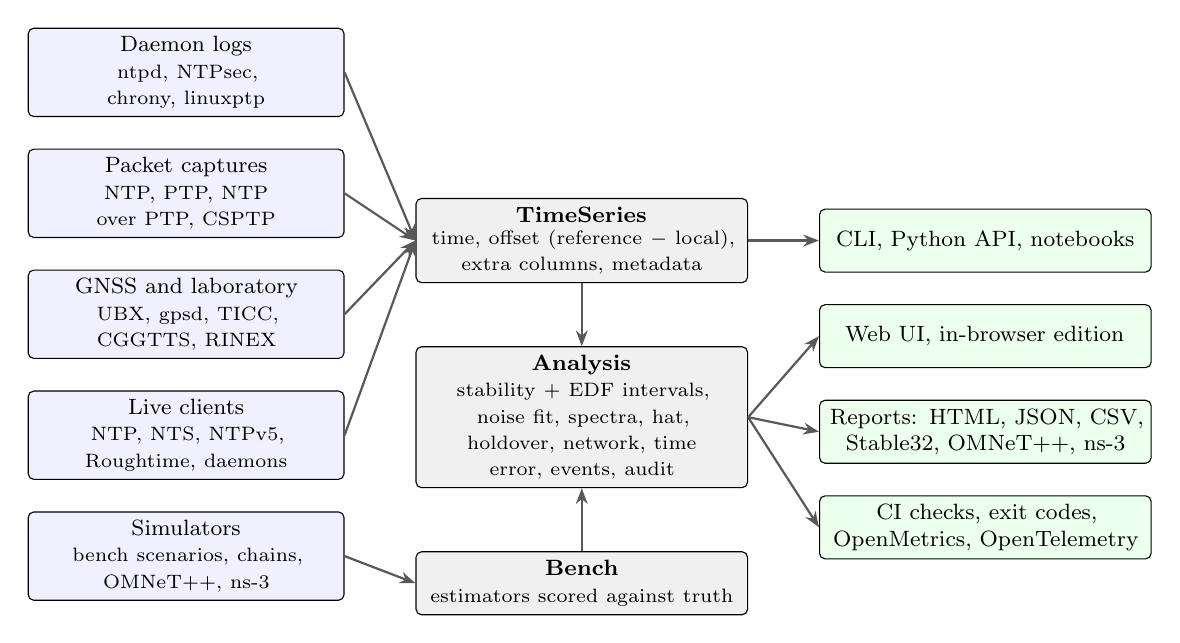
\begin{tikzpicture}[
  node distance=4mm and 6mm,
  box/.style={draw, rounded corners=2pt, align=center, font=\footnotesize, execute at begin node={\hyphenpenalty=10000\relax\exhyphenpenalty=10000\relax}, minimum height=8mm, inner sep=3pt},
  src/.style={box, fill=blue!6, text width=38mm},
  core/.style={box, fill=gray!12, text width=40mm},
  outp/.style={box, fill=green!7, text width=40mm},
  arr/.style={-{Stealth[length=2mm]}, thick, gray!70!black}]
\node[src] (logs) {Daemon logs\\{\scriptsize ntpd, NTPsec, chrony, linuxptp}};
\node[src, below=of logs] (caps) {Packet captures\\{\scriptsize NTP, PTP, NTP over PTP, CSPTP}};
\node[src, below=of caps] (gnss) {GNSS and laboratory\\{\scriptsize UBX, gpsd, TICC, CGGTTS, RINEX}};
\node[src, below=of gnss] (live) {Live clients\\{\scriptsize NTP, NTS, NTPv5, Roughtime, daemons}};
\node[src, below=of live] (sim) {Simulators\\{\scriptsize bench scenarios, chains, OMNeT++, ns-3}};
\node[core, right=9mm of caps, yshift=-6mm] (ts) {\textbf{TimeSeries}\\{\scriptsize time, offset (reference $-$ local),\\ extra columns, metadata}};
\node[core, below=8mm of ts] (an) {\textbf{Analysis}\\{\scriptsize stability + EDF intervals, noise fit, spectra, hat, holdover, network, time error, events, audit}};
\node[core, below=8mm of an] (bench) {\textbf{Bench}\\{\scriptsize estimators scored against truth}};
\node[outp, right=9mm of ts] (cli) {CLI, Python API, notebooks};
\node[outp, below=of cli] (ui) {Web UI, in-browser edition};
\node[outp, below=of ui] (rep) {Reports: HTML, JSON, CSV,\\ Stable32, OMNeT++, ns-3};
\node[outp, below=of rep] (ci) {CI checks, exit codes,\\ OpenMetrics, OpenTelemetry};
\foreach \n in {logs,caps,gnss,live} \draw[arr] (\n.east) -- (ts.west);
\draw[arr] (sim.east) -- (bench.west);
\draw[arr] (ts) -- (an);
\draw[arr] (bench.north) -- node[right, font=\scriptsize]{} (an.south);
\draw[arr] (an.east) -- (rep.west);
\draw[arr] (an.east) -- (ci.west);
\draw[arr] (ts.east) -- (cli.west);
\draw[arr] (an.east) -- (ui.west);
\end{tikzpicture}
\caption{Structure of \ntp. Every input is converted to one series type with one sign convention; the
analysis and the bench operate only on that type, and every result is available through the
command line, the Python API, the web interface and machine-readable reports.}\label{fig:architecture}
\end{figure}

\section{Validation}\label{sec:validation}

\subsection{Published reference values}\label{sec:nist}

NIST SP~1065 \citep[sec.~12]{riley2008} publishes two test suites: the nine-point frequency data of NBS
Monograph~140 (its Table~30, at averaging factors 1 and 2) and a 1000-point series generated by the
linear congruential recursion $n_{i+1} = 16807\,n_i \bmod (2^{31}-1)$ from $n_0 = 1234567890$ (Table~31,
at factors 1, 10 and 100). Both are regenerated in the test suite and in the experiment script. The
values printed in the handbook have seven significant digits. \Cref{tab:nist} lists the largest relative
deviation of \ntp{} from the printed values for every statistic in the tables; all are below the
$5\times10^{-7}$ that the rounding of seven digits allows, and the largest is $2.8\times10^{-7}$ (TDEV,
1000-point suite). HTOT, which the handbook tabulates with a noise-dependent bias correction, agrees to
within 0.3\% in the test suite; we do not count it as an exact reproduction.

\begin{table}[t]
\centering\small
\caption{Largest relative deviation of \ntp{} from the values printed in NIST SP~1065, Tables 30 and 31.
The tables give seven significant digits, so deviations below $5\times10^{-7}$ are rounding.}\label{tab:nist}
\begin{tabular}{@{}lcc@{}}
\toprule
Statistic & NBS 9-point ($m = 1, 2$) & 1000-point ($m = 1, 10, 100$) \\
\midrule
\rows{tables/nist.tex}
\bottomrule
\end{tabular}
\end{table}

\subsection{Coverage of confidence intervals}\label{sec:coverage}

Agreement with tables checks the point estimates, not their uncertainty. To check the intervals, we
simulated 400 records of 1025 phase points for each of the five power-law noise types, computed OADEV
and MDEV with 95\% intervals at $m = 1, 4, 16, 64$, and counted how often the interval contained the
expected deviation of the generating model. The noise type was identified from each record, as a user
would do. \Cref{fig:coverage} shows the result next to the coverage of the common shortcut
$\sigma \pm 1.96\,\sigma/\sqrt{n}$.

With 400 runs, the standard error of an observed coverage near 0.95 is about 0.011. With the exact
EDF the coverage lies between 0.91 and 0.98 in 38 of the 40 cases, and between 0.93 and 0.97 in 34. The shortcut is
adequate only at $m = 1$ and, for OADEV, under white PM; elsewhere its coverage falls to between 0.24
and 0.6 at $m = 64$, because overlapping terms are strongly correlated. The exception for the EDF
method is flicker PM with OADEV at large $m$ (0.87 at $m = 16$ and 0.70 at $m = 64$, against 0.93 and
0.92 for MDEV). For this noise type the Allan deviation depends only weakly on $\tau$ and the lag-1
estimate of the noise type becomes ambiguous on short records, so a wrong EDF model is chosen in part of
the runs. MDEV, which separates white and flicker PM, does not show the problem. We report this as a
limitation: users who expect flicker PM should prefer MDEV or TDEV, which is also the recommendation of
the time-and-frequency literature \citep{riley2008}.

\begin{figure}[t]
\centering
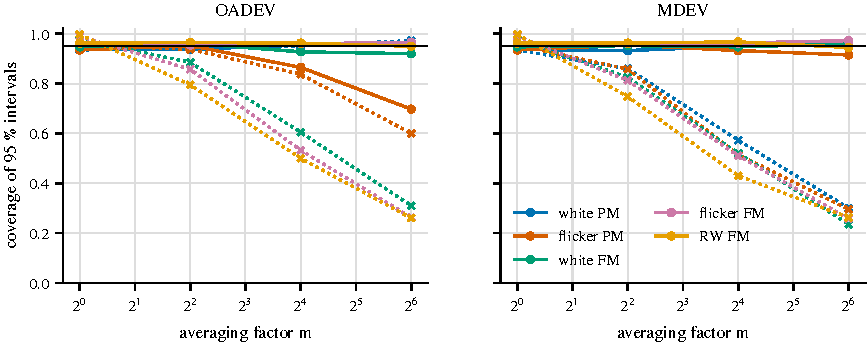
\includegraphics[width=\linewidth]{figures/ci-coverage.pdf}
\caption{Share of 400 simulated records in which the 95\% interval contains the true deviation.
Solid: $\chi^2$ intervals with the exact discrete EDF and the noise type identified from each record.
Dotted: the shortcut $\sigma \pm 1.96\,\sigma/\sqrt{n}$. The horizontal line marks 0.95.}\label{fig:coverage}
\end{figure}

Further tests, which we summarise without repeating their numbers, check every estimator against a
literal implementation of its formula and against the analytic slopes of the five noise types; check
the EDF against Monte Carlo variances; check the coverage of the noise-model intervals, the N-cornered
hat and the holdover envelope; compare against a frozen table of values from an independent
implementation (\texttt{allantools}, stored as data, not a dependency); and exercise the protocol
clients against local test servers, including Kiss-o'-Death packets, spoofed and forged responses,
certificate mismatches and the NTP era rollover of 2036.

\subsection{A silent error in practice}\label{sec:legacy}

The 2012 prototype of this project is preserved unchanged in the repository, together with the ntpd
\texttt{loopstats} file it was developed with. That file has 52 samples written at the poll interval,
with a median spacing of 1072~s and a gap of 2.6~h. The prototype's Allan deviation routine assumed a
spacing of 32~s regardless of the data and treated the samples as evenly spaced. \Cref{fig:legacy}
compares its output with \ntp. The prototype reports $\sigma_y = 8.6\times10^{-4}$ at $\tau = 32$~s.
Rescaling to the actual spacing moves both axes by a factor of $1072/32 = 33.5$, which gives
$2.6\times10^{-5}$ at 1072~s; \ntp, which in addition does not bridge the gap, gives
$4.9\times10^{-6}$ with a 68\% interval of $[4.5, 5.5]\times10^{-6}$. With 52 samples the curve says
little about this clock, but the case shows how a plausible-looking stability plot can be wrong by two
orders of magnitude when the sampling is assumed rather than read from the data.

\begin{figure}[t]
\centering
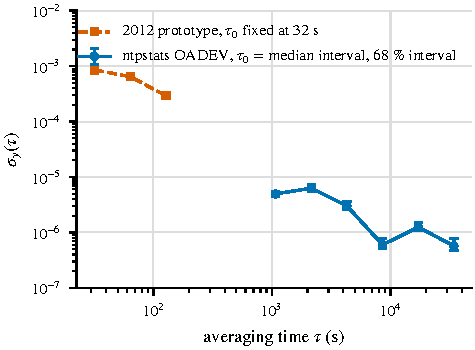
\includegraphics[width=0.62\linewidth]{figures/legacy-adev.pdf}
\caption{Stability of the 2012 sample \texttt{loopstats} file: the 2012 prototype, which fixed
$\tau_0 = 32$~s, against \ntp{} OADEV with the median interval, gaps left open and 68\% intervals.}\label{fig:legacy}
\end{figure}

\section{Experiments}\label{sec:experiments}

All results in this section are produced by \texttt{experiments.py} and \texttt{make\_tables.py},
published with this paper, from \ntp{} 3.5.0 with fixed seeds.

\subsection{Estimators on simulated NTP networks}

\Cref{tab:bench} reports the RMS error of the single-server estimators on four of the bundled
scenarios, over five seeds. \texttt{lan} is a local network (16~s polling, 80\us{} propagation each
way, tens of microseconds of queueing, 6~h); \texttt{internet} is a wide-area path (64~s polling, 5\ms{}
propagation each way, 1 and 3\ms{} mean queueing, 24~h); \texttt{congested} has 20\ms{} propagation and
8 and 15\ms{} mean queueing with 2\% loss; \texttt{route-change} adds a 4\ms{} step of the forward
propagation delay after 8~h, an evening congestion period and a temperature cycle of the oscillator.

\begin{table}[t]
\centering\small
\caption{RMS error of the offset estimate (\micro s), mean $\pm$ standard deviation over five seeds,
excluding the first 30~minutes. Single-server estimators, scored on the first server.}\label{tab:bench}
\begin{tabular}{@{}lrrrr@{}}
\toprule
Estimator & \texttt{lan} & \texttt{internet} & \texttt{congested} & \texttt{route-change} \\
\midrule
\rows{tables/bench-ntp.tex}
\bottomrule
\end{tabular}
\end{table}

Three observations stand out. First, on paths whose two directions have the same floor, the choice of
estimator matters by two orders of magnitude: on \texttt{internet} the raw offsets have an RMS error of
1.6\ms{}, the NTP clock filter 118\us{}, regression and feed-forward estimators about 55\us{}, and the
Huygens-style hull 11\us. The hull uses the bound $\theta \pm \delta/2$ of every exchange, not only the
lowest-delay ones, which is why it gains most where queueing is heavy (13\us{} on \texttt{congested},
against 575\us{} for the next best). Second, PTP-style servos tuned for hardware time stamps on a
local network (\texttt{ptp4l}, \texttt{sptp}) follow the delay variation of a wide-area path and are
worse than the raw offsets there; they are included as references for the PTP experiments below, not
as NTP clients. Third, no estimator survives the route change. After the step, every estimator settles
at an error of about 2\ms{}, half of the 4\ms{} one-way step: the median error between 10 and 18~h,
averaged over five seeds, is 2.00\ms{} for the clock filter, 1.99\ms{} for the hull and between 1.71
and 1.92\ms{} for the others. This is the asymmetry limit of \cref{eq:ntp} made visible: the error is in
the path, and no two-way estimator can see it.

The \texttt{falseticker} scenario has four servers: one with a constant 40\ms{} error and one that steps
by 100\ms{} after 12~h, both larger than the root distance of about 10\ms. \Cref{tab:falseticker} shows
that the RFC~5905 selection and the intersection-based combination reject them, whereas the median of
the four clock-filter outputs follows them once two of the four servers are wrong. A single-server
estimator on a correct server is, in this scenario, better still; the value of the selection algorithms
lies in not knowing which server that is.

\begin{table}[t]
\centering\small
\caption{Multi-server estimators on \texttt{falseticker} (five seeds): RMS error (\micro s) and largest absolute error (ms).}\label{tab:falseticker}
\begin{tabular}{@{}lrr@{}}
\toprule
Estimator & RMS (\micro s) & max (ms) \\
\midrule
\rows{tables/bench-falseticker.tex}
\bottomrule
\end{tabular}
\end{table}

\subsection{PTP exchanges and clients}

The \texttt{ptp-lan} scenario models a PTP slave behind switches without PTP support: one Sync and one
Delay\_Req per second, 8\ns{} time-stamp noise, 4\us{} propagation, and mean queueing of 3\us{} towards
the slave and 6\us{} towards the master with loads of 0.4 and 0.5. \texttt{ptp-tc} is the same network
with transparent clocks that correct 95\% of the queueing. \Cref{fig:ptp} and \cref{tab:ptp} show the
RMS error over three seeds of four hours.

\begin{figure}[t]
\centering
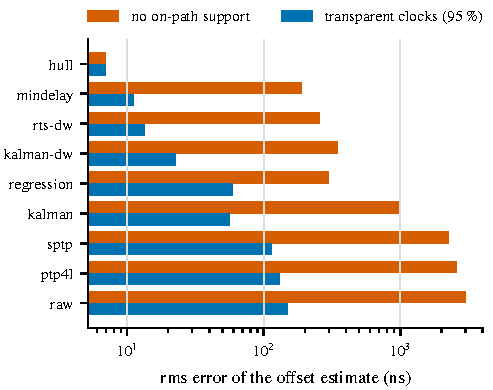
\includegraphics[width=0.62\linewidth]{figures/ptp-bench.pdf}
\caption{RMS error of the offset estimate on exchange-level PTP, without on-path support and with
transparent clocks that correct 95\% of the queueing (three seeds, 4~h each).}\label{fig:ptp}
\end{figure}

\begin{table}[t]
\centering\small
\caption{RMS error (ns) on exchange-level PTP, three seeds of 4~h.}\label{tab:ptp}
\begin{tabular}{@{}lrr@{}}
\toprule
Estimator & \texttt{ptp-lan} & \texttt{ptp-tc} \\
\midrule
\rows{tables/bench-ptp.tex}
\bottomrule
\end{tabular}
\end{table}

With linuxptp's default gains at one Sync per second, the modelled \texttt{ptp4l} servo follows the
packet delay variation: without on-path support it improves on the raw offsets by only 13\%, and
transparent clocks reduce its error twentyfold, from 2.6\us{} to 129\ns. Estimators that use the delay
of every exchange do far better on the same packets: the clock filter reaches 187\ns{} without on-path
support, and the hull estimator 7\ns{} in both cases, which is close to the time-stamp noise. The
comparison has a caveat. The hull assumes that the two directions have equal floors, which holds in
this scenario by construction; a constant asymmetry would bias it, like every two-way method. Within
that assumption, the result supports the case for delay-filtering PTP clients and for carrying NTP over
PTP, where corrections and hardware time stamps can be combined with a client-side estimator.

\subsection{Time error along boundary-clock chains}

We simulated chains of 20 boundary clocks at 16 Sync and 16 Delay\_Req messages per second for one
hour, with three servo configurations and three seeds each: the PI servo with linuxptp's default gains
for hardware time stamping, the PI servo with a narrow loop ($k_p = 0.3$~s$^{-1}$, $k_i = 3.5\times10^{-4}$
per sample, a bandwidth of about 0.05~Hz), and the linear-regression servo. The warm-up excluded from the
metrics is derived from the slowest pole of the loop, with a minimum of 300~s.

\begin{figure}[t]
\centering
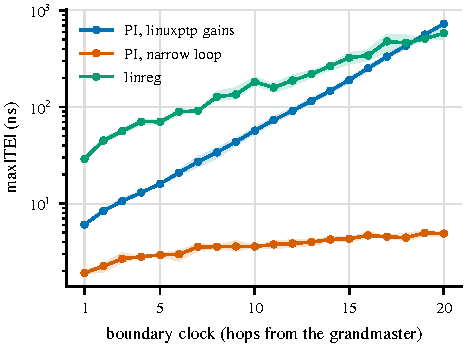
\includegraphics[width=0.62\linewidth]{figures/chain-maxte.pdf}
\caption{max|TE| of each boundary clock along a 20-hop chain (mean of three seeds; the band spans the
seeds). Default linuxptp gains show gain peaking: the error grows much faster than the number of
hops.}\label{fig:chain}
\end{figure}

\begin{table}[t]
\centering\small
\caption{Boundary-clock chains of 20 hops: max|TE| (ns) at hops 1, 5, 10 and 20, MTIE of
dTE$_\mathrm{L}$ at hop 20 (ns), and the warm-up excluded (s). Mean of three seeds.}\label{tab:chains}
\begin{tabular}{@{}lrrrrrr@{}}
\toprule
Servo & 1 & 5 & 10 & 20 & MTIE$_{20}$ & warm-up \\
\midrule
\rows{tables/chains.tex}
\bottomrule
\end{tabular}
\end{table}

\Cref{fig:chain} and \cref{tab:chains} show the effect known as gain peaking. With the default gains,
which are chosen for a single slave, each loop amplifies part of the wander it receives; cascaded, the
peaks multiply, and max|TE| grows from 6\ns{} at the first hop to 57\ns{} at the tenth and 728\ns{} at
the twentieth. A narrow, well-damped loop keeps the twentieth hop at 4.9\ns, at the price of a longer
lock time (the excluded warm-up rises from 300 to 1250~s). The regression servo starts with a larger
error (29\ns{} at the first hop) but grows more slowly, and at twenty hops it ends close to the default
PI servo (581\ns).
Under these assumptions (no asymmetry, no packet delay variation between boundary clocks, and
oscillators with identical noise parameters), the default configuration uses two thirds of the
1.1\us{} budget of G.8271.1 at twenty hops before any asymmetry is counted, whereas the narrow loop
leaves almost all of it for asymmetry and other error sources. The
model is not a product: real boundary clocks have their own servos and filters. What the simulation
provides is a controlled way to see how servo bandwidth, message rates, asymmetry and noise interact
along a chain, and to check a design against a budget before building it.

\subsection{Public servers}\label{sec:interop}

A weekly workflow on GitHub-hosted runners queries public servers with every client, and the first
run of each month is added to an open dataset in the repository, archived with each release. The run
of 30 September 2026 (ntpstats 2.13.0, IPv4, \cref{tab:interop}) illustrates what the data contain. All
six NTPv4 servers and all five NTS servers answered; each NTS server returned a fresh cookie per
exchange (eight cookies left after two exchanges); none of the six servers probed answered in
interleaved mode, and none of four servers probed offered NTPv5. Three of the four Roughtime servers
answered and one timed out; the NTS pool test failed because the experimental pool's name did not
resolve. In every NTP and NTS measurement, $|\theta|$ was between 0.2\% and 40\% of $\delta/2$, so all
offsets are compatible with a correct server and an asymmetric path. A single run is a snapshot, not a
measurement of the servers' accuracy; the value of the dataset is in its growth and its openness.

\begin{table}[t]
\centering\small
\caption{Single exchanges from one GitHub-hosted runner (30 September 2026). $\theta$ is the server
minus the runner clock; the last column compares $|\theta|$ with the asymmetry bound $\delta/2$.}\label{tab:interop}
\begin{tabular}{@{}llrrrr@{}}
\toprule
Test & Server & Stratum & $\theta$ (ms) & $\delta$ (ms) & $|\theta|/(\delta/2)$ \\
\midrule
\rows{tables/interop.tex}
\bottomrule
\end{tabular}
\end{table}

\subsection{Computational cost}

On one core of the machine used for this paper (x86-64, Python 3.13, NumPy 2.5), OADEV, MDEV, HDEV
and TOTDEV of a record of $10^6$ phase points at octave-spaced averaging times, each with noise
identification and EDF-based intervals, took between 1.0 and 1.4~s. The complete experiment script
runs in about ten minutes.

\section{Discussion}\label{sec:discussion}

\paragraph{What the toolkit does not claim.} The estimators and servos are models written from published
descriptions, not the daemons' code; their numbers characterise algorithms under stated conditions, not
products. The simulator's path model (a fixed floor with exponential queueing) is deliberately simple;
trace replay is the way to bring real delay distributions into the bench, and it inherits the
unobservability of a constant asymmetry. Parsers for vendor instruments rely on declarative profiles
until sample exports are contributed. The validation reproduces published tables and checks interval
coverage by simulation, but a comparison with Stable32 output files on further data sets, including its
confidence intervals, has not been done yet, nor a long comparison of real logs against an independent
reference such as a GNSS-disciplined host.

\paragraph{Threats to validity.} The experiments use simulated networks whose parameters were chosen to
be representative, not measured; results on real networks can differ, which is why the bench accepts
replayed traces. The coverage study uses one record length (1025 points) and four averaging factors;
the flicker PM shortfall shows that the identification step, not the EDF itself, can limit coverage on
short records. The public-server table is a single run from one location.

\paragraph{Why one toolkit.} Most of the functions described here exist somewhere, in a stability
program, a daemon, an instrument or a paper's evaluation code. Putting them on one data model has
practical consequences that go beyond convenience. The sign convention is fixed once, so a chrony
tracking log, a PTP capture and a counter export can be compared directly. The same statistics, with
the same intervals, are applied to a deployment log and to an algorithm's output on simulated truth, so
a result in the field and a result in a paper can be related. And because the bench, the scenarios and
the seeds are open, a claim that an algorithm improves on another can be checked by anyone.

\section{Availability and reproducibility}\label{sec:availability}

\ntp{} is available under the MIT licence from PyPI (\texttt{pip install ntpstats}), with source, documentation and issue tracker at
\url{https://github.com/thiagodefreitas/NetworkTime} and documentation at
\url{https://thiagodefreitas.github.io/NetworkTime/}. Each release is archived on Zenodo
\citep{ntpstats}. The \LaTeX{} source of this paper, the experiment script, the generated data and the
figures are in the directory \texttt{research/preprint-2026} of the repository. To reproduce every number:
\begin{verbatim}
pip install ntpstats==3.5.0 matplotlib
python research/preprint-2026/experiments.py
python research/preprint-2026/make_tables.py
\end{verbatim}

\section*{Acknowledgements}

\ntp{} began as a Google Summer of Code 2012 project for the NTP Project of the Network Time
Foundation. The author thanks the maintainers of the protocols, daemons, standards and open data sets
on which this work builds.

\bibliographystyle{unsrtnat}
\bibliography{refs}

\end{document}
